\documentclass{article}

\usepackage{pdfsync}
\usepackage{natbib}
\usepackage{hyperref}
\usepackage{graphicx}
\usepackage{caption}
\usepackage{subcaption}

% dot graphs
\usepackage{dot2texi}
\usepackage{tikz}
\usetikzlibrary{shapes,arrows}

\begin{document}
	\author{Robin Deits\\ rdeits@csail.mit.edu}
	\title{6.375 Report: Adaptive PIV: Synthesis}
	\date{\today}
	\maketitle

	\tableofcontents

	\section{Background: PIV} % (fold)
	\label{sec:background}
	Particle Image Velocimetry (PIV) is an optical approach to measuring the flow field of a fluid, and has been used in the study of combustion, water flow, robotics, and many other fields. It involves seeding a fluid with tracking particles and using a laser or other planar lighting system to capture sequential images of the particle positions in a single thin 2D slice of the fluid. By comparing the change in position of groups of particles between the subsequent frames, a measurement of the local flow vector can be computed for each region of the fluid. This process of determining the movement of each section of the image is extremely time-consuming in a sequential programming system, but can be readily parallelized to significantly improve performance \citep{Yu:2006tb}

	Each PIV computation is performed on a pair of sequential images. Computation of the fluid flow begins by dividing the image up into small windows of, for example, 64px on a side. A small window size helps ensure that all of the particles within the window move with the same velocity between the two frames. For each window, we extract the subimage corresponding to that window from the first image in the pair. We will call this subimage $A$. We then extract a set of subimages $B_{\Delta x,  \Delta y}$ by shifting the original window in two dimensions and extracting the corresponding subimages from the second image in the pair. We can then perform a cross-correlation between $A$ and each $B_{i, j}$ and determine the shift in $x$ and $y$ which maximizes the correlation. This gives the most likely location of the particles from window $A$ in the second frame, and thus indicates the movement of that section of the fluid between the frames.
	% section background (end)

	\section{Adaptive PIV} % (fold)
	\label{sec:adaptive_piv}
	Standard PIV algorithms involve an even spatial distribution of interrogation windows $A$ with a fixed window size and some fixed overlap, such as 64\,px windows beginning every 16\,px. However, in order to achieve sufficient accuracy in busy fluid flows, it can be necessary to choose very small windows or very high degrees of overlap, which increases the computational demands by requiring far more cross-correlation computations. 	Theunissen et al. proposed a method for improving the performance of PIV in sub-optimial conditions, called Adaptive PIV \citep{Theunissen:2009cr}. Their method uses information about the current density of seeding particles and the prior estimate of the velocity field to update the size and spatial frequency of the interrogation windows $A$. This has the effect of increasing the number of data points in the busiest (highest particle density and highest velocity) parts of the fluid and reducing the number of samples in the most stable areas of the fluid, which can improve the amount of relevant data collected per computational unit. 

	In this project, I will focus on implementing Adaptive PIV on an FPGA to improve computational performance, with the ultimate goal of allowing accurate real-time fluid tracking. I will be expanding on prior work implementing a standard PIV algorithm on an FPGA \citep{Yu:2006tb}. I will also be using a recent \textsc{Matlab} implementation of the Adaptive PIV algorithm by Samvaran Sharma of the Robot Locomotion Group at MIT CSAIL as the reference code for my implementation. 

	The primary benefit of this project should be the parallelization and speedup of the Adaptive PIV algorithm. In order to achieve the desired image size and accuracy, Sharma's current software requires approximately 2.5 seconds per pair of frames, which makes real-time analysis of the fluid flow impossible. In contrast, Yu et al. were able to compute 15 image pairs per second using their FPGA implementation. My goal will be to achieve this result with the added benefits of the adaptive algorithm's focus on the most important areas of the fluid flow.
	% section adaptive_piv (end)

	\section{Implementation}
	I will divide the implementation of the PIV system up into the high-level logic, which will be performed in Python, and the computationally intensive and parallelizable cross-correlation which will be performed on the FPGA. This division is shown in Figure~\ref{fig:system}. The host machine will read image pairs from disk (simulating live capture from a camera system), then convert them to 4-bit grayscale. These image pairs will be transmitted over SCEMI to the FPGA, which will store both images in DRAM. The host machine will then select a series of interrogation windows. The exact method of selection will depend on whether we are performing normal or adaptive PIV. The host will transmit the coordinates of the interrogation windows to the DUT. The FPGA will then extract the actual image data for each window, perform the cross-correlation, and locate the peak in the cross-correlation value signifying the displacement of the particles in the window. The FPGA will then send the displacement back to the host. 

	\subsection{Module: Window Tracker}
	The FPGA will contain many instances of the Window Tracker module, each of which will perform the cross-correlation and displacement extraction for a single interrogation window. The Window Tracker will be implemented as a server with the following operations: 
	\begin{enumerate}
		\item put(x, y): begin calculating the cross-correlation and displacement for a new window located at (x, y) in the image
		\item u, v = get(): get the displacement of the interrogation window which was previously input to put()
	\end{enumerate}
	The Window Tracker will have a number of submodules, described below:

	\subsubsection{Module: Window Manager}
	The Window Manager will be responsible for extracting the correct pixel values from the images stored in the DRAM. It needs to support the following operations: 
	\begin{enumerate}
		\item reset(x, y): begin extracting pixels for a new interrogation window located at the point (x, y) in the first image
		\item px = getNextPixel(): return the value of the next pixel needed for cross-correlation computation. Since the order in which pixel values are accessed is fixed, this function needs no input.
	\end{enumerate}
	The fixed access order for pixel values used in the cross-correlation algorithm means that we can easily make the Window Manager's access to the DRAM fully pipelined, and we can also cache values from the DRAM to reduce the number of memory accesses.

	\subsubsection{Module: Accumulator}
	The Accumulator will take pixel values from the Window Manager and compute a running sum of the product of its pairs of inputs. It will automatically reset its internal total to zero for each element in the cross-correlation matrix output.
	\begin{enumerate}
		\item update(px1, px2): add px1 * px2 to the internal total. This total is copied to result and then reset to zero after every $c$ calls to update(), where $c$ is the number of multiplications and additions required per element in the cross-correlation matrix
		\item result = get(): Return result and then set result to Invalid
	\end{enumerate}

	\subsubsection{Module: Tracker}
	The Tracker determines from the output of the Accumulator the current displacement values with the highest cross-correlation between the windows. It polls the get() method of the Accumulator and maintains internal variables for the highest result seen so far and the x and y displacements corresponding to it. Once all cross-correlation computations are finished, it makes its result available. 
	\begin{enumerate}
		\item x\_disp, y\_disp = get(): Return the displacement in x and y of the peak of the cross-correlation matrix.
	\end{enumerate}


\begin{figure}[htbp]
\makebox[\textwidth][c]{
	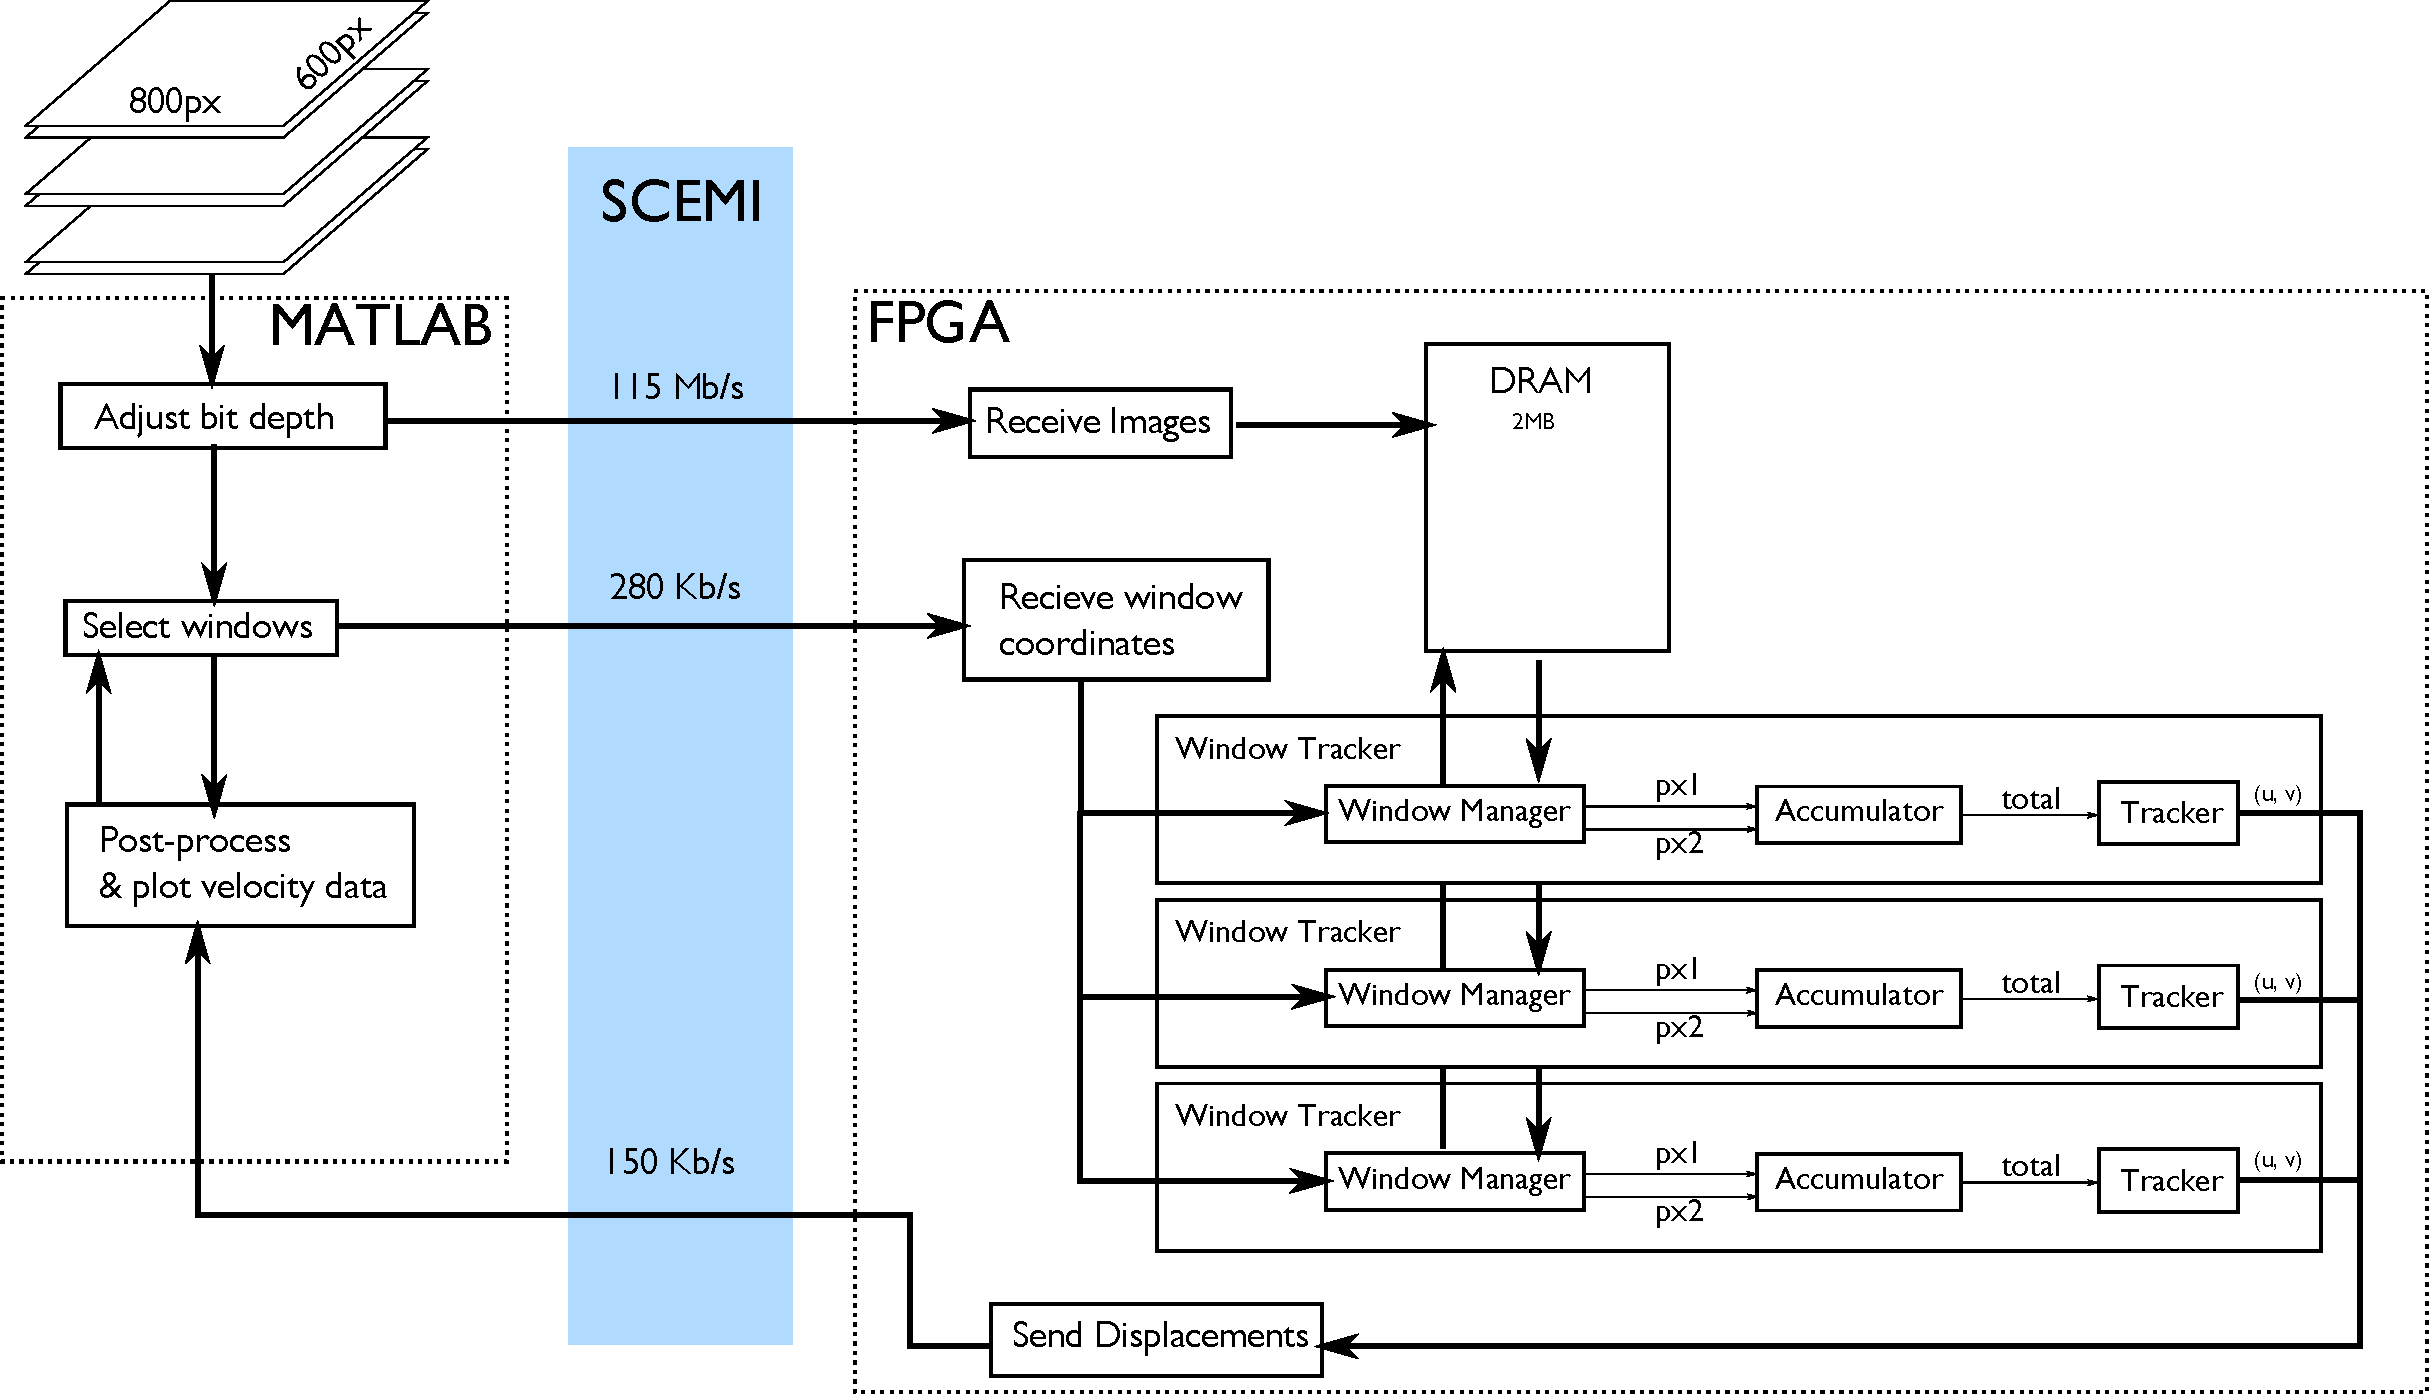
\includegraphics[width=1.4\textwidth]{system_diagram.pdf}}
	\caption{The system diagram for the Adaptive PIV implementation on the FPGA. High-level logic relating to the particular PIV implementation is performed in Python, and the cross-correlation is performed on the FPGA. Only 3 Window Tracker modules are shown, but the full implementation should have up to 40 or more.}
	\label{fig:system}
\end{figure}

\section{Computational Requirements}
In order to assess the computational requirements of this design, I chose to use the interrogation window parameters presented by Yu et al. \citep{Yu:2006tb}. This choice means an interrogation window of 40x40px for the first image in each pair and 32x32px for the second image in each pair. For clarity, we will refer to the images as Image A and Image B and the frames as Frame A (40x40) and Frame B (32x32). Cross-correlation will be performed for each fully overlapping position of Frame B within Frame A. This means that the cross-correlation matrix will have $(40 - 32 + 1) ^2 = 81$ elements. 

Each element in the cross-correlation matrix will require $32 * 32$ multiplications and additions, so the entire cross-correlation matrix will require $32 * 32 * 81 = 82944$ multiplications. To compute the full velocity vector field for normal PIV, using an 8 pixel shift between interrogation windows, we must compute 1680 cross-correlation matrices per image pair. This means that, for a throughput of 15 image pairs per second, we need to perform $2,090,188,800$ multiplications per second. At a clock speed of 50\,MHz, that comes down to approximately 40 multiplications per clock cycle, meaning that the final design will need 40 Window Tracker modules each performing a single multiplication per cycle. 
\section{Testing Plan}
I will use the sample data provided with Sharma's Adaptive PIV implementation, which consists of simulated image pairs of a vortex flow. I will compare the displacements calculated by the FPGA implementation to those produced by Sharma's cross-correlation code using the same window size settings and also compare the execution speed of the normal PIV algorithm with publicly available PIV implementations. My specific goals are:
\begin{enumerate}
	\item 15 image pairs per second throughput
	\item Cross-correlation results which exactly match those produced by \textsc{Matlab}
\end{enumerate}

\section{Implementation Status}
As of Apr. 29, I have implemented the complete PIV system in simulation. I have created a simple Python script which loads in a pair of 800x600\,px images, transmits their pixel data to the simulated FPGA test bench, and then sends requests for 40\,px windows spaced every 8\,px. The Python program then displays the velocity vector field received for each window. 

\subsection{Demonstration}
To test the PIV system, I generated several small image pairs with known displacements. By applying an 80x60\,px window to a source image, and then shifting that window by a few pixels in a given direction, I created pairs of images with perfectly uniform, controlled displacements, which the PIV system was able to accurately track. One such pair is shown in Figure \ref{fig:diag_test}. 

In addition, I have run the PIV system in simulation on an entire 800x600\,px image pair, using the test set from Sharma's adaptive PIV system. The results are shown  in Figure \ref{fig:full_test}. 

\begin{figure}
	\centering
	\begin{subfigure}[htb]{0.45\textwidth}
		\centering
		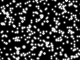
\includegraphics[width=\textwidth]{../../data/test/x+2_y+2/A.png}
	\end{subfigure}
	\begin{subfigure}[htb]{0.45\textwidth}
		\centering
		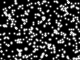
\includegraphics[width=\textwidth]{../../data/test/x+2_y+2/B.png}
	\end{subfigure}

	\begin{subfigure}[htb]{.7\textwidth}
		\centering
		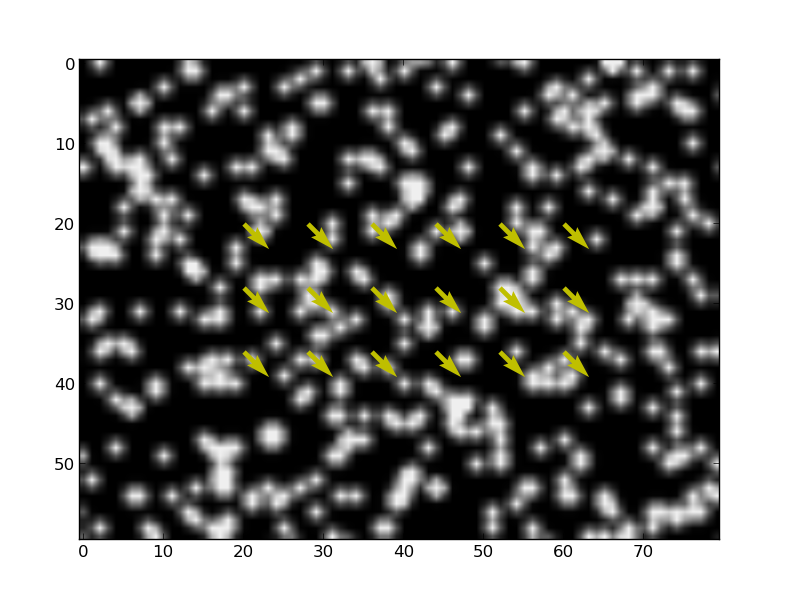
\includegraphics[width=\textwidth]{../../data/test/x+2_y+2/PIV.png}
	\end{subfigure}
	\caption{A pair of sample images created to test the PIV system. The image on the upper left has been shifted down and to the right by two pixels to create the image on the upper right. The lower image shows the calculated flow field from the PIV program, which matches this displacement.}
	\label{fig:diag_test}
\end{figure}

\begin{figure}
	\centering
	\begin{subfigure}[htb]{0.45\textwidth}
		\centering
		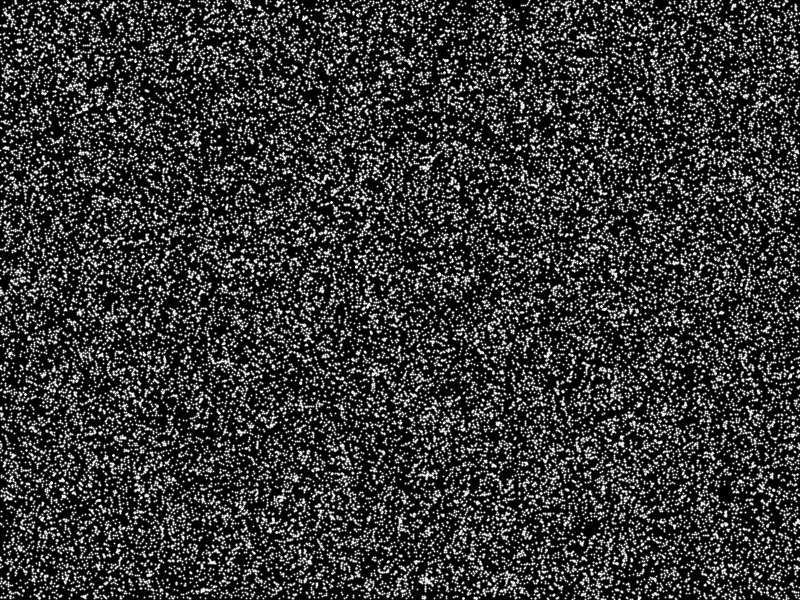
\includegraphics[width=\textwidth]{../../data/vort_sim/A.png}
	\end{subfigure}
	\begin{subfigure}[htb]{0.45\textwidth}
		\centering
		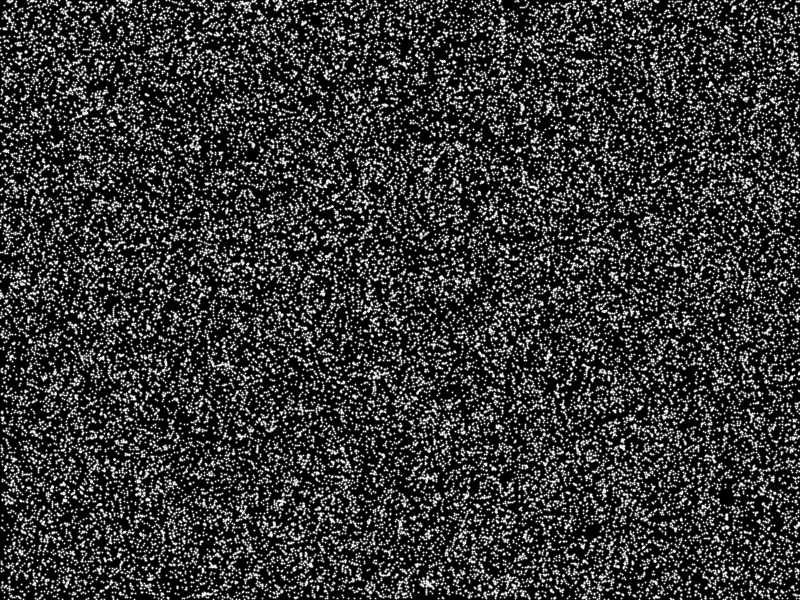
\includegraphics[width=\textwidth]{../../data/vort_sim/B.png}
	\end{subfigure}

	\begin{subfigure}[htb]{\textwidth}
		\centerline{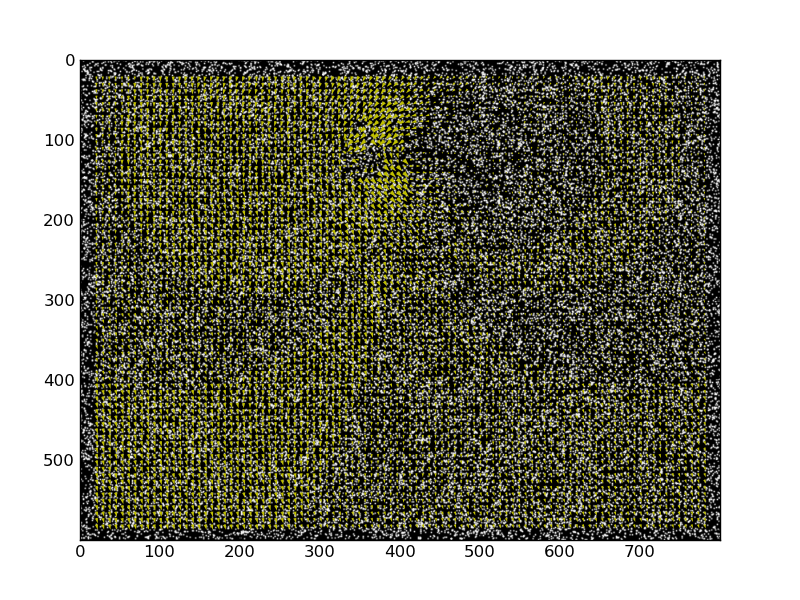
\includegraphics[trim = .4in .4in .4in .4in, clip, width=1.5\textwidth]{../../data/vort_sim/PIV.png}}
	\end{subfigure}
	\caption{A pair of full-size synthetic images taken from Sharma's adaptive PIV system, along with the measured flow field from the simulated FPGA implementation.}
	\label{fig:full_test}
\end{figure}

\section{Explorations}
\subsection{Variable Window Size}
If possible, I would like to extend the design to support varying the size of the interrogation window. This is an important part of the Adaptive PIV algorithm, as it allows the system to examine smaller windows of particle flow in busy areas of the image, in which the assumption that all particles within a window are moving with the same velocity might not hold for a larger window. This will require adding a window size parameter to the reset() method of the Window Manager and will require that that size parameter be passed to the Accumulator and Tracker in order to adjust their behavior accordingly. 

\subsection{Image Data Caching}
I suspect that contention for BRAM access among all the Window Managers will be a major difficulty as I attempt to parallelize my design. I plan to explore several variables related to this problem: 
\begin{itemize}
	\item Memory data size: wider memory data will allow more pixel values to be received per read of the BRAM, but may create timing problems.
	\item Caching image data: each window manager may need to cache the pixel values of its interrogation windows. As of Apr. 22, I have implemented this in my design.
	\item Number of BRAM ports: adding memory ports will allow for more parallel reads, but may create other resource issues.
\end{itemize}

	\bibliographystyle{plain}
	\bibliography{refs}
\end{document}